\section{簡介}
%文獻上已經提出許多改進資料不足語言的句法剖析的方法,其中多半需要該資料不足語言的特性,用以找尋與其相似的語言進行協同訓練。
%近年來初見於影像領域的模型無關元學習,本來是為了處理少量樣本學習的問題,
%不久後也為資料不足(但資料量大於少量樣本學習)的學習任務所用\cite{gu-etal-2018-meta},
%不需要事先知道任務的特性,

\iffalse
有名的語言學家杭氏(Noam Chomsky)觀察人類習得語言的過程,
他認為嬰孩學習語言時所接收到的語言輸入是不足以讓他們習得該語言的所有特徵的,
許多特性相異的語法都可以產生這些他們所接收到的語料,
但孩童仍然習得了該語言的正確語法,
因此他推斷人類出生時大腦中即具備有某種語言習得裝置(Language acquisition device),
而語言習得裝置的任務便是從所有與語料匹配的語法中挑選正確的語法
\fi
本章介紹使用模型無關元學習進行多語言預訓練,以幫助資料不足語言的依存句法剖析的系列實驗。

模型無關元學習,本來是為了處理圖片分類領域少量樣本學習的問題,
不久後也為資料不足(但資料量大於少量樣本學習)的學習任務所用,
如古氏(Jiatao Gu)將元學習方法引入資料不足的機器翻譯,
並勝過使用普通多語言學習的基準模型\cite{gu-etal-2018-meta}。
芬氏(Chelsea Finn)在2018年提出的模型無關元學習(model-agnostic meta-learning)
\cite{Finn2017ModelAgnosticMF}為所有使用梯度下降法(gradient descent)進行最佳化的模型的提供了一項簡潔且有效的方法處理資料不足任務。
在語言轉移學習的框架下,其目標是替未見過的語言(unseen languages)尋找一合適參數初始值,使得少量步數梯度更新後,參數在該語言的測試集上表現最佳,
其稱此在少量步數更新就能大幅增進爲見過語言表現的能力為「快速適應」(fast adaptation)。
%其強調使用少量步數進行梯度更新,即是由於資料不足語言資料稀少,過多步數容易過擬合。

在元學習出現以前,
若希望利用相似語言中所蘊含的資訊給予模型語言普遍具備的歸納偏置(下稱普適語言偏置,universal linguistic biases),
多語言學習(multilingual learning)為一主要的方法\cite{caruana1997multitask}。
藉由共享特徵抽取網路並用以同時訓練多種相關語言,
相關語言的資訊得以透過反向傳播(backpropagation)注入類神經網路中,
使模型相較於解釋單一語言,更加偏好能夠解釋所有相關語言的假說,
有效幫助模型達成泛化(generalization)。

然而多語言訓練的目標,是提高訓練語言(training languages)在其測試集(testing set)上的準確率,
而提高訓練語言的準確率,未必就代表在資料不足語言上的準確率也會隨之提高;
有可能出現訓練語言與資料不足語言差異過大,而導致多語言訓練模型無法幫助資料不足語言的任務表現。

不若單純的多語言訓練,模型無關元學習於訓練階段的目標並非提高在訓練語言上的表現,
而是直接最佳化模型在未見過語言上\finetune後的表現,訓練與測試環境沒有不匹配之處,
希望減輕模型只在訓練語言的測試集上有好表現,而無法推廣到資料不足語言上的問題。

本章為了了解模型無關元學習及其各種一階近似的變形(見第\ref{sec:mamls}節)在多語言依存句法剖析上的行為,
去除詞的影響,只使用詞性標記作為特徵進行依存句法剖析。
另外,為了更深入了解不同模型組態(model configurations)對於模型無關元學習系列方法的影響,
也以模型大小為操作變因,試圖了解小模型與大模型是否會改變不同方法對依存句法剖析的表現。
最後,藉由觀察不同方法經過不同精細校正階段後在目標語言方向性分佈的改變軌跡,
試圖分析模型無關元學習是否有達到其宣稱的快速適應的能力。
\iffalse
尤其當目標任務缺乏資料的時候,若使用過於有表現力的假說集合,
易使模型過擬合到目標任務上,
利用相似任務進行多工學習幫助目標任務提升表現的效果尤其顯著。
然而多工學習得到的模型可以在訓練過的所有任務上的測試集有好表現,
但並未保證這樣的好表現可以轉移到相似但未見過的任務上;
而芬氏(Chelsea Finn)提出的模型無關元學習(model-agnostic meta-learning)
\cite{Finn2017ModelAgnosticMF}提供了多工學習之外的另一種方法,
將領域的歸納偏置(inductive bias)注入類神經網路中。
\fi

\section{多語言去詞化依存句法剖析(multilingual delexicalized dependency parsing)}
由於詞化依存句法剖析有太多變因,包括使用的預訓練模型,其對不同語言的偏置等等,都會影響句法剖析模型於目標語言上的行為;
且詞化依存句法剖析參數量較多,使用二次微分的計算量與佔用空間均較大,訓練耗時,
有時甚至會發生用來進行平行矩陣運算的圖形處理器記憶體不足的問題。
因此為了排除語言本身句法以外性質對句法剖析的影響及計算資源的考量,
本節先進行去詞化依存句法剖析的實驗,
也就是只使用句法樹庫提供的詞性標記做為詞的表徵進行句法剖析,
詞化依存句法剖析留待第\ref{chapter:lex_parsing}章再行探討。

\subsection{詞性標記(POS tags)}
UD句法樹庫中大部分的語言均提供兩種詞性標記:專為該語言設計的詞性標記(XPOS),通常為該句法樹庫尚未整合進UD時原本的詞性標記,
與各語言統一的普適詞性標記\cite{petrov-etal-2012-universal}(Universal POS tags, UPOS),
其捨棄各語言細緻的詞性分別,
整合語言間相似性質的詞性,以達到所有語言共享同一組詞性集合的目標。
如前置介系詞(prepositions)與後置介系詞(postpositions)在UPOS的框架下就被整合成介系詞(adpositions)而不做前後置之分。
由於UPOS有更好的跨語言通用性,本研究去詞化依存句法剖析的詞性標記輸入均使用UPOS。

\subsection{修訂版爬蟲類元學習}
原始版本的爬蟲類元學習\cite{nichol2018first}無論是在內循環或外循環的開頭都不會重新啟動內循環的優化器,
當使用有動能(momentum)的優化器如Adam時,當下的梯度更新會受之前用其他語言計算而得的梯度影響,
造成語言間不必要的干擾。
為了避免此現象,原作者將一階動能項$\beta_{1}$設為$0$。
%然而mBERT原始論文中進行精細校正使用的為具有動能項的Adam,
然而初始實驗發現$\beta_{1} = 0$的Adam在精細校正時時會對準確率造成負面影響。
再者,爬蟲類元學習將外循環原始梯度(raw gradient)直接設為各語言內循環(亦即精細校正)前後參數的差異的平均,
此數值大小很大程度上取決於內循環優化器的學習率,
恐與一般模型精細校正時接收到的梯度分佈差異過大。

為處理此問題,本研究稍稍修改了爬蟲類元學習的演算法,
希望在不改變內循環優化器設置的前提下保留爬蟲類元學習加總內循環所有梯度的優點:
與其將內循環梯度設為前後參數的差異的平均 $\phi - U_{\textrm{ADAM}}^{k}(\phi) $,
內循環原始梯度經過內循環優化器處理過後的產物,
本研究將內循環梯度直接設為內循環\textbf{原始}梯度的平均(此處優化器以Adam為例):
\begin{equation}
    g_{\textrm{REP}} = \mathbb{E}_{\tau}\left[ \frac{1}{k} \sum_{i=1}^{k} \nabla_{\phi_{i}} \mathcal{L}_{\tau} \left( \phi_{i}^{\texttt{adam}} \right) \right]
\end{equation}
其中
\begin{equation}
    \phi_{i}^{\texttt{adam}} = U_{\textrm{ADAM}} \left( \phi_{i - 1}^{\texttt{adam}} \right).
\end{equation}
此數值雖然是由內循環優化器計算出來,但此處取其原始梯度,
受內循環學習率影響較小。
此修訂版爬蟲類元學習與普通的多語言學習的差異比起原始的爬蟲類元學習要來的更小:
外循環的梯度為內循環原始梯度的平均,與多語言學習類似;
但原始梯度仍是由內循環更新過的參數計算出來的(除了內循環的第一步),更接近原本的爬蟲類元學習。
初始實驗發現此修訂版爬蟲類元學習表現不俗,
且相較原始爬蟲類元學習的表現來的更加穩定。
本研究稍稍濫用爬蟲類元學習的名稱,往後皆以爬蟲類元學習指稱本節所提出的修訂版爬蟲類元學習。

\section{實驗設置}
\label{sec:delex_depparse_setting}
\begin{table}[h!]
\centering
\begin{subtable}[t]{.5\textwidth}
    \begin{tabular}[t]{|l l|}
        \hline
        \textbf{語言} & \textbf{句法樹庫編碼} \\
        \hline
        Afrikaans & af\_afribooms \\
        Ancient Greek & grc\_proiel \\
        Ancient Greek & grc\_perseus \\
        Arabic & ar\_padt \\
        %Armenian & hy\_armtdp \\
        Basque & eu\_bdt \\
        Bulgarian & bg\_btb \\
        %Buryat & bxr\_bdt \\
        Catalan & ca\_ancora \\
        Chinese & zh\_gsd \\
        Croatian & hr\_set \\
        Czech & cs\_cac \\
        Czech & cs\_fictree \\
        Czech & cs\_pdt \\
        Danish & da\_ddt \\
        Dutch & nl\_alpino \\
        Dutch & nl\_lassysmall \\
        English & en\_ewt \\
        English & en\_gum \\
        English & en\_lines \\
        Estonian & et\_edt \\
        Finnish & fi\_ftb \\
        Finnish & fi\_tdt \\
        French & fr\_gsd \\
        French & fr\_sequoia \\
        French & fr\_spoken \\
        Galician & gl\_ctg \\
        Galician & gl\_treegal \\
        German & de\_gsd \\
        Gothic & got\_proiel \\
        Greek & el\_gdt \\
        Hebrew & he\_htb \\
        Hindi & hi\_hdtb \\
        Hungarian & hu\_szeged \\
        Indonesian & id\_gsd \\
        %Irish & ga\_idt \\
        \hline
    \end{tabular}
\end{subtable}%
\begin{subtable}[t]{.5\textwidth}
    \begin{tabular}[t]{|l l|}
        \hline
        \textbf{語言} & \textbf{句法樹庫編碼} \\
        \hline
        Italian & it\_isdt \\
        Italian & it\_postwita \\
        Japanese & ja\_gsd \\
        %Kazakh & kk\_ktb \\
        Korean & ko\_gsd \\
        Korean & ko\_kaist \\
        %Kurmanji & kmr\_mg \\
        Latin & la\_ittb \\
        Latin & la\_proiel \\
        Latin & la\_perseus \\
        Latvian & lv\_lvtb \\
        %North Sami & sme\_giella \\
        Norwegian & no\_bokmaal \\
        Norwegian & no\_nynorsk \\
        Norwegian & no\_nynorsklia \\
        Old Church Slavonic & cu\_proiel \\
        Old French & fro\_srcmf \\
        Persian & fa\_seraji \\
        Polish & pl\_lfg \\
        Polish & pl\_sz \\
        Portuguese & pt\_bosque \\
        Romanian & ro\_rrt \\
        Russian & ru\_syntagrus \\
        Russian & ru\_taiga \\
        Serbian & sr\_set \\
        Slovak & sk\_snk \\
        Slovenian & sl\_ssj \\
        Slovenian & sl\_sst \\
        Spanish & es\_ancora \\
        Swedish & sv\_lines \\
        Swedish & sv\_talbanken \\
        Turkish & tr\_imst \\
        Ukrainian & uk\_iu \\
        %Upper Sorbian & hsb\_ufal \\
        Urdu & ur\_udtb \\
        Uyghur & ug\_udt \\
        Vietnamese & vi\_vtb \\
        \hline
    \end{tabular}
\end{subtable}
\caption{預訓練所使用的訓練句法樹庫/語言。}
\label{tab:training_languages}
\end{table}
% \begin{table}[h!]
% \centering
% \begin{subtable}[t]{.5\textwidth}
%     \centering
%     \begin{tabular}[t]{|l l|}
%         \hline
%         \textbf{語言} & \textbf{句法樹庫編碼} \\
%         \hline
%         Buryat & bxr\_bdt \\
%         Kurmanji & kmr\_mg \\
%         Upper Sorbian & hsb\_ufal \\
%         Armenian & hy\_armtdp \\
%         Kazakh & kk\_ktb \\
%         Irish & ga\_idt \\
%         North Sami & sme\_giella \\
%         \hline
%     \end{tabular}
%     \caption{真實資料不足測試句法樹庫/語言。}
%     \label{tab:true_lr_testing_languages}
% \end{subtable}%
% \begin{subtable}[t]{.5\textwidth}
%     \centering
%     \begin{tabular}[t]{|l l|}
%         \hline
%         \textbf{語言} & \textbf{句法樹庫編碼} \\
%         \hline
%         Wolof & wo\_wtb \\
%         Scottish Gaelic & gd\_arcosg \\
%         Coptic & cop\_scriptorium \\
%         Telugu & te\_mtg \\
%         Belarusian & be\_hse \\
%         Marathi & mr\_ufal \\
%         Maltese & mt\_mudt \\
%         Tamil & ta\_ttb \\
%         \hline
%     \end{tabular}
%     \caption{模擬資料不足測試句法樹庫/語言。}
%     \label{tab:sim_lr_testing_languages}
% \end{subtable}%
% \caption{資料不足測試句法樹庫/語言。}
% \end{table}

\begin{table}[h!]
\centering
    \begin{tabular}[t]{|l l|}
        \hline
        \textbf{語言} & \textbf{句法樹庫編碼} \\
        \hline
        Wolof & wo\_wtb \\
        Scottish Gaelic & gd\_arcosg \\
        Coptic & cop\_scriptorium \\
        Telugu & te\_mtg \\
        Belarusian & be\_hse \\
        Marathi & mr\_ufal \\
        Maltese & mt\_mudt \\
        Tamil & ta\_ttb \\
        \hline
    \end{tabular}
    \caption{測試用未見過的句法樹庫/語言。}
    \label{tab:unseen_languages}
\end{table}
\begin{table}[htbp]
    % \fontsize{8}{10}\selectfont
    \centering
    \begin{subtable}[t]{.4\textwidth}
        \centering
        \begin{tabular}[t]{@{}lr@{}}
        \toprule
        超參數 & 值 \\
        \midrule
            詞性嵌入維度         & 100 \\
            詞性嵌入維度(小模型) & 10 \\
            編碼器              & 雙向LSTM \\
            編碼器層數           & 3 \\
            編碼器隱維度         & 100 \\
            編碼器隱維度(小模型) & 10 \\
            依存邊維度           & 200 \\
            依存邊維度(小模型)   & 20 \\
            依存標籤維度          & 200 \\
            依存標籤維度(小模型) & 20 \\
            詞性丟棄機率            & 0.33 \\
            批次大小$b$         & 16 \\
            語言數$l$           & 10 \\
            訓練樣本數/回合        & 64000 \\
            訓練回合數          & 10 \\
            優化器              & Adam \\
            $\beta_1,\beta_2$  & 0.9, 0.9 \\
            權重衰減參數         & 0.01 \\
            基礎學習率          & $3e^{-4}$ \\
            最大梯度範數        & 5.0 \\
            內循環步數          & 2 \\
        \bottomrule
        \end{tabular}
        \caption{
            預訓練超參數。
        }
        \label{tab:delex_pretrain_hparams}
    \end{subtable}
    \hspace{10pt}
    \begin{subtable}[t]{.4\textwidth}
        \centering
        \begin{tabular}[t]{@{}lr@{}}
        \toprule
        超參數 & 值 \\
        \midrule
            優化器              & Adam \\
            基礎學習率          & $3e^{-4}$ \\
            $\beta_1,\beta_2$  & 0.9, 0.9 \\
            批次大小            & 16 \\
            訓練回合數          & 80 \\
            最大梯度範數        & 5.0 \\
        \bottomrule
        \end{tabular}
        \caption{
            精細校正超參數。
        }
        \label{tab:delex_finetune_hparams}
    \end{subtable}
    \caption{
        去詞化依存句法剖析模型超參數一覽。
    }
    \label{tab:delex_hparams}
\end{table}
我們從\conll的53種訓練語言(73個訓練句法樹庫)中選取有官方驗證集(development set)的46種訓練語言(66個訓練句法樹庫)作爲訓練語言;見表\ref{tab:training_languages}。
預訓練完成後,我們分別對該模型進行\zeroshot及\finetune在預訓練中未見過的語言上。
%我們挑選\conll的訓練語言中剩下的只有訓練集而沒有發展集的語言作爲真實資料不足測試語言(true low-resource testing languages,見表\ref{tab:true_lr_testing_languages})。
%為了觀察控制資料多寡時對不同預訓練方法的影響,
%我們另外挑選了UD 2.5版中8種不在訓練語言中的語言做為模擬資料不足測試語言(simulated low-resource testing languages,見表\ref{tab:sim_lr_testing_languages})。
我們挑選UD 2.5版中8種不在訓練語言中的語言做為測試用的未見過語言(unseen languages,見表\ref{tab:unseen_languages})。
實驗在訓練與測試時時均使用正確的斷句、斷詞,並使用句法樹庫提供的正確詞性做為詞的表徵。

至於多語言訓練的部分,孔氏\cite{kondratyuk-straka-2019-75}與烏氏\cite{ustun2020udapter}進行多語言訓練的方法,
是將全部語言的句法樹庫接在一起、在一個小批次(batch)中混合多個句法樹庫訓練。
這樣的做法可能會導致資料量大的語言取樣頻率過高;
我們的方法則是每次更新從全部語言裡取樣$l$種語言,每種語言取樣$b$個句子,一個批次總共有$b \times l$個句子。
不同於孔氏與烏氏,這樣的方法防止模型過度對資料充足語言的特性建模,但也可能使得資料不足語言的句子被過度取樣而產生過擬合的現象。

超參數的設置見表\ref{tab:delex_hparams}。
\section{實驗結果}
以下首先呈現去詞化依存句法剖析的實驗結果,
\subsection{去詞化依存句法剖析}
\begin{figure}[htbp]
    \centering
    \begin{subfigure}[t]{\textwidth}
        \centering
        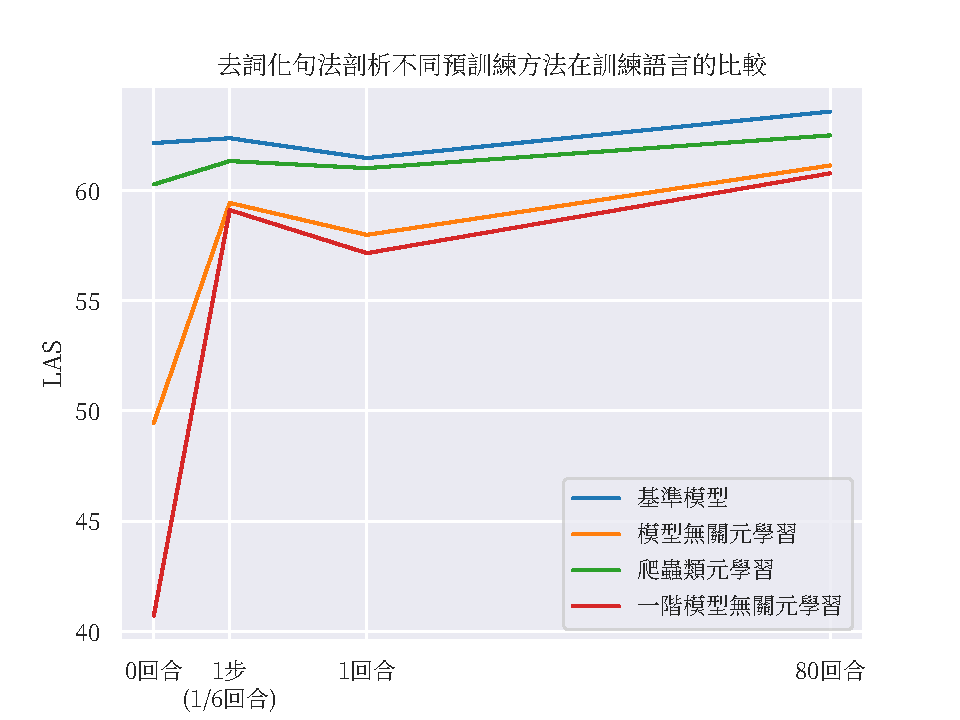
\includegraphics[width=\textwidth]{figs/delex_parsing/linecharts/delex_train_langs.pdf}
    \end{subfigure}
    \vspace{-12pt}
    \begin{subfigure}[t]{\textwidth}
        \centering
        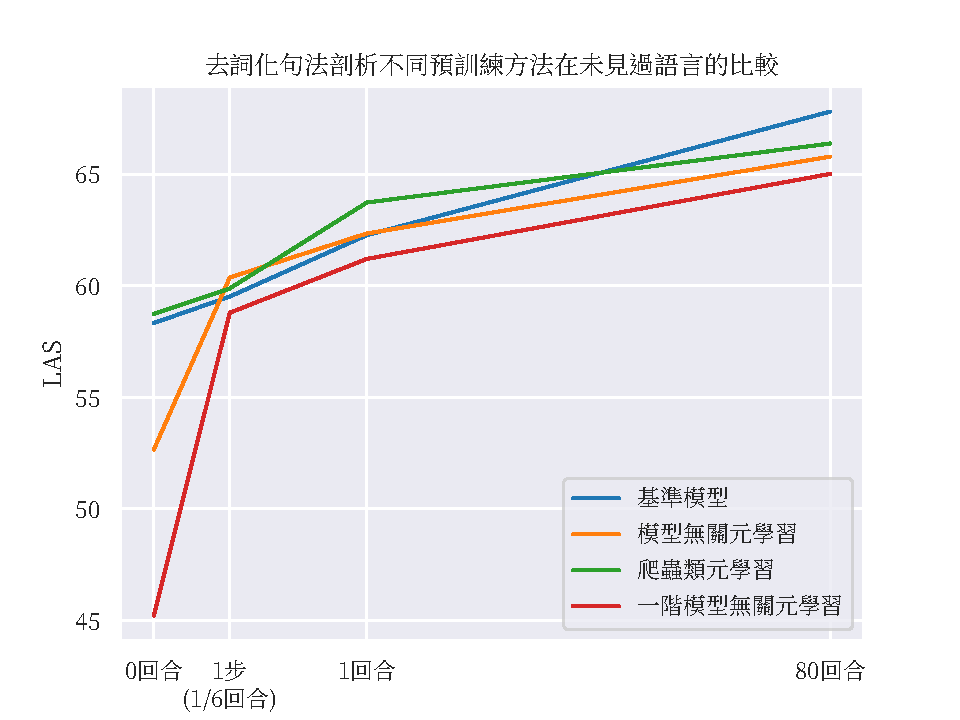
\includegraphics[width=\textwidth]{figs/delex_parsing/linecharts/delex_test_langs.pdf}
    \end{subfigure}
    \caption{去詞化依存句法剖析不同預訓練方法精細校正後的平均LAS折線圖。}
    \label{fig:delex_avg}
\end{figure}
\begin{figure}[htbp]
    \centering
    \begin{subfigure}[t]{0.8\textwidth}
        \centering
        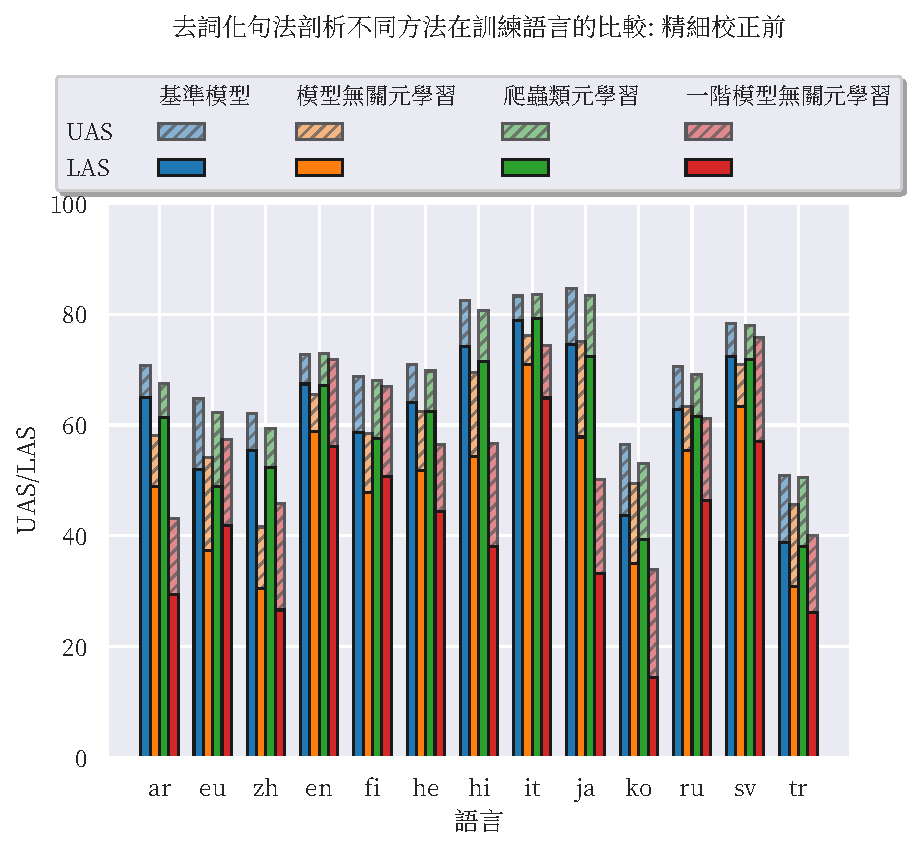
\includegraphics[width=\textwidth]{figs/delex_parsing/barplots/bar_zs_train_langs.pdf}
    \end{subfigure}
    \vspace{-12pt}
    \begin{subfigure}[t]{0.8\textwidth}
        \centering
        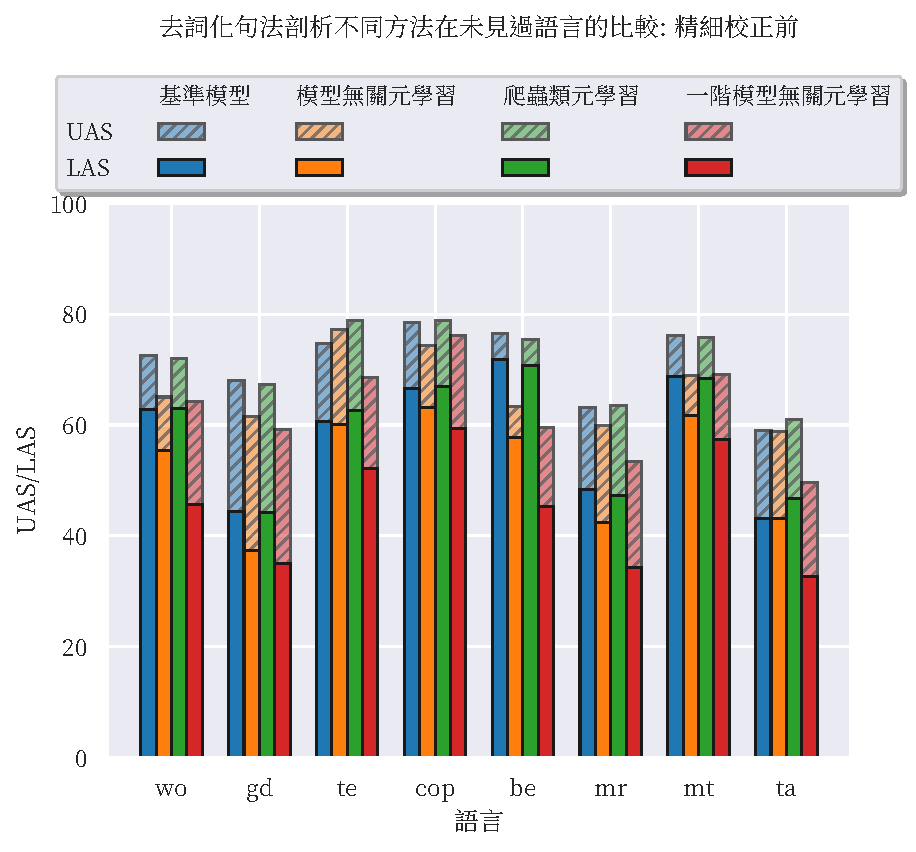
\includegraphics[width=\textwidth]{figs/delex_parsing/barplots/bar_zs_test_langs.pdf}
    \end{subfigure}
    \caption{去詞化依存句法剖析不同方法在各語言精細校正前的UAS/LAS長條圖。}
    \label{fig:bar_zs}
\end{figure}
\begin{figure}[htbp]
    \centering
    \begin{subfigure}[t]{0.8\textwidth}
        \centering
        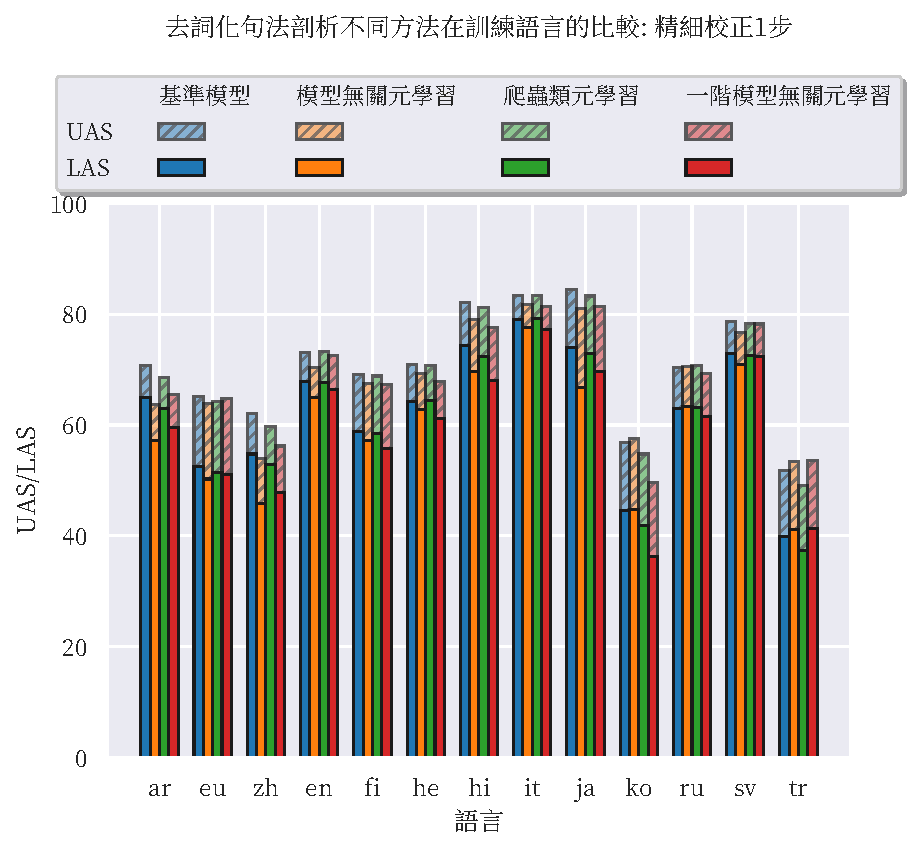
\includegraphics[width=\textwidth]{figs/delex_parsing/barplots/bar_one_step_train_langs.pdf}
    \end{subfigure}
    \vspace{-12pt}
    \begin{subfigure}[t]{0.8\textwidth}
        \centering
        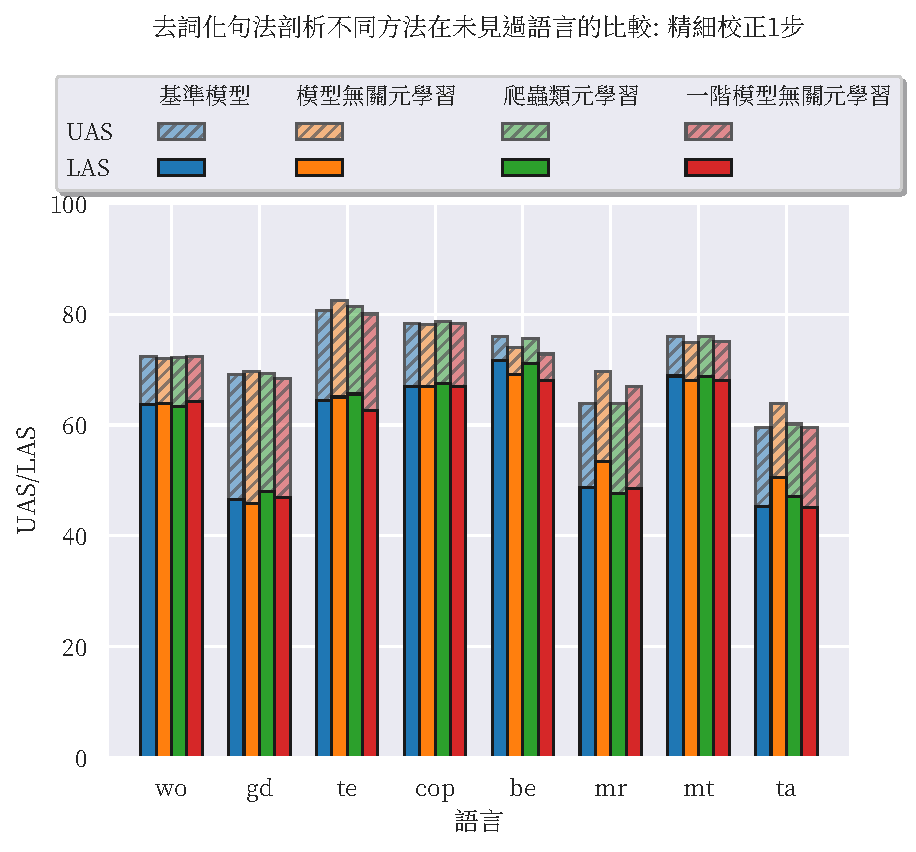
\includegraphics[width=\textwidth]{figs/delex_parsing/barplots/bar_one_step_test_langs.pdf}
    \end{subfigure}
    \caption{去詞化依存句法剖析不同方法在各語言精細校正一步($\frac{1}{6}$回合)後的UAS/LAS長條圖。}
    \label{fig:bar_one_step}
\end{figure}
\begin{figure}[htbp]
    \centering
    \begin{subfigure}[t]{0.8\textwidth}
        \centering
        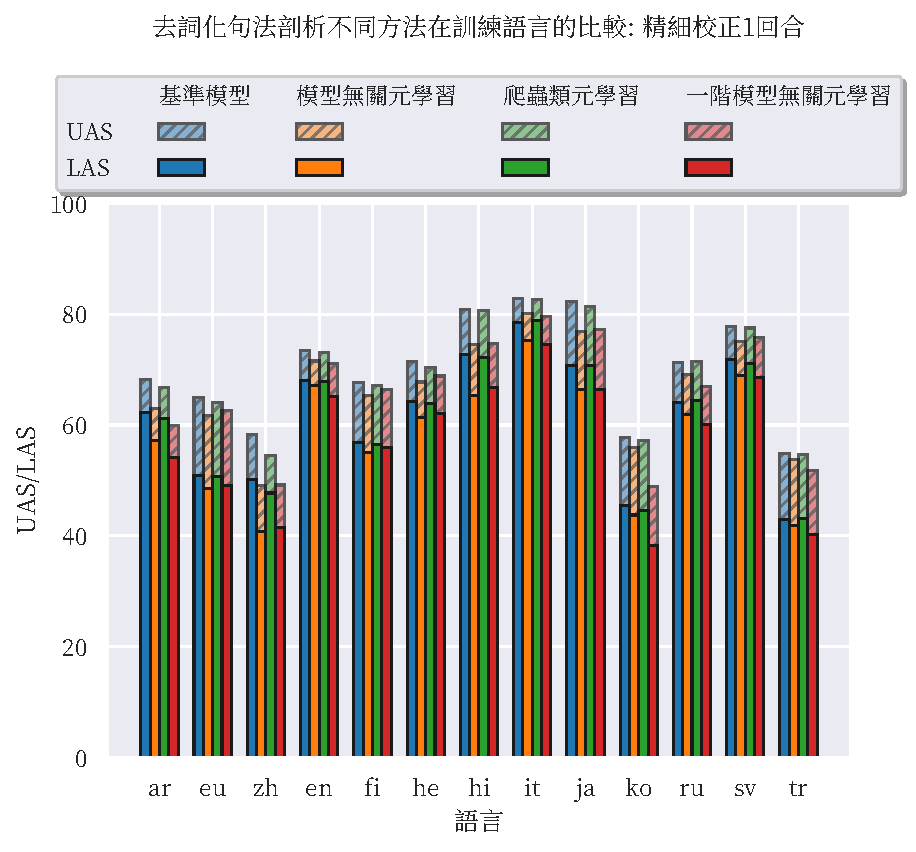
\includegraphics[width=\textwidth]{figs/delex_parsing/barplots/bar_full_epoch_1_train_langs.pdf}
    \end{subfigure}
    \vspace{-12pt}
    \begin{subfigure}[t]{0.8\textwidth}
        \centering
        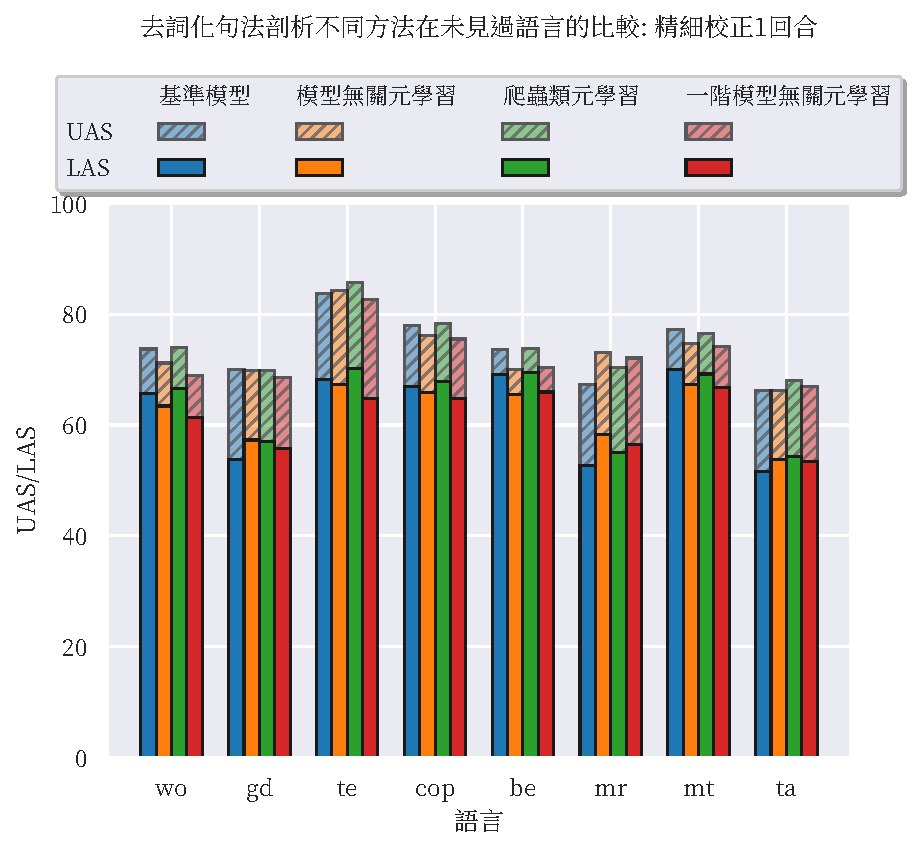
\includegraphics[width=\textwidth]{figs/delex_parsing/barplots/bar_full_epoch_1_test_langs.pdf}
    \end{subfigure}
    \caption{去詞化依存句法剖析不同方法在各語言精細校正一回合後的UAS/LAS長條圖。}
    \label{fig:bar_full_epoch_1}
\end{figure}
\begin{figure}[htbp]
    \centering
    \begin{subfigure}[t]{0.8\textwidth}
        \centering
        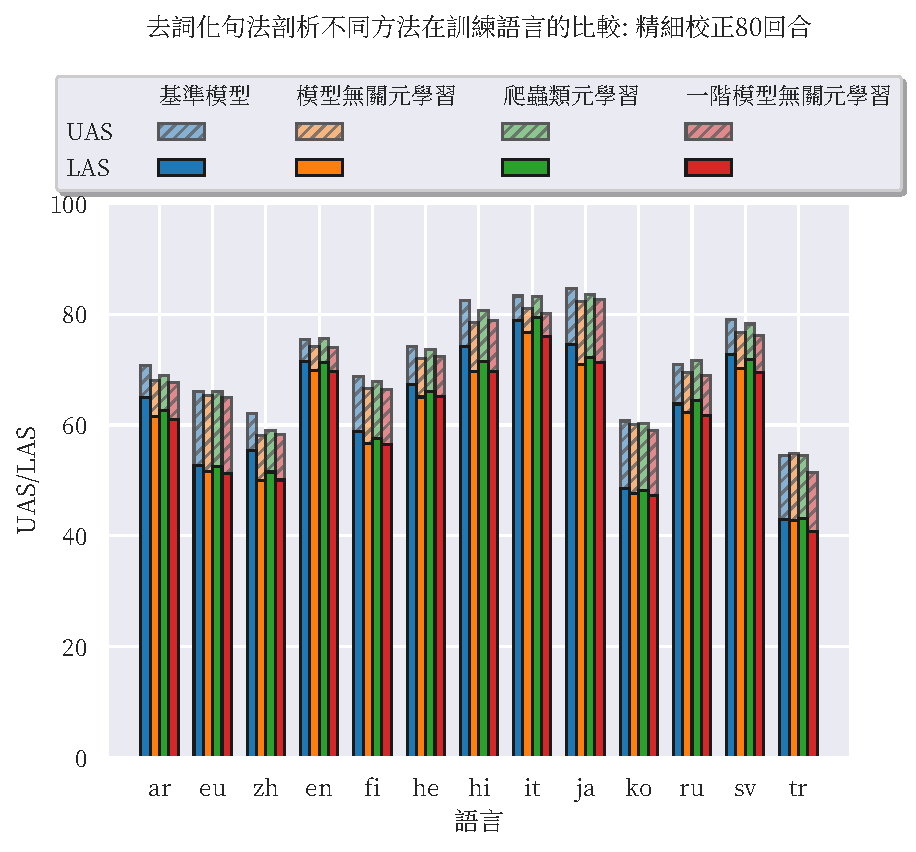
\includegraphics[width=\textwidth]{figs/delex_parsing/barplots/bar_full_epoch_80_train_langs.pdf}
    \end{subfigure}
    \vspace{-12pt}
    \begin{subfigure}[t]{0.8\textwidth}
        \centering
        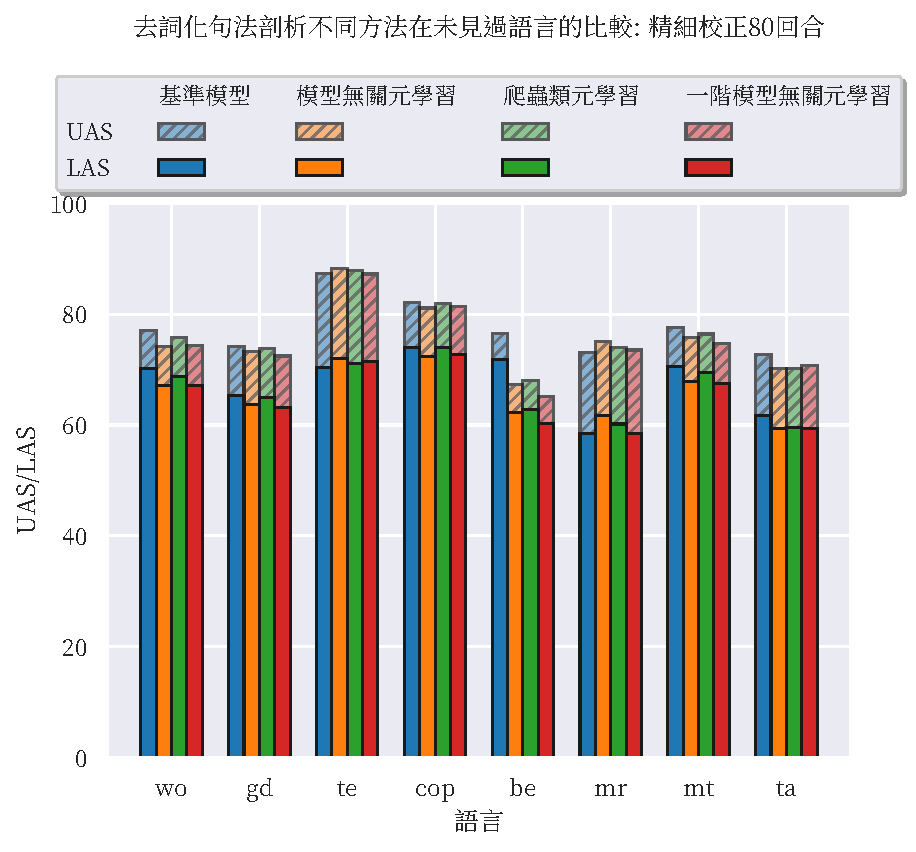
\includegraphics[width=\textwidth]{figs/delex_parsing/barplots/bar_full_epoch_80_test_langs.pdf}
    \end{subfigure}
    \caption{去詞化依存句法剖析不同方法在各語言精細校正八十回合後的UAS/LAS長條圖。}
    \label{fig:bar_full_epoch_80}
\end{figure}
\begin{figure}[htbp]
    \centering
    \begin{subfigure}[t]{0.7\textwidth}
        \centering
        \includegraphics[width=\textwidth]{figs/delex_parsing/dir_scatterplots/zs_train_langs.pdf}
    \end{subfigure}
    \vspace{-12pt}
    \begin{subfigure}[t]{0.7\textwidth}
        \centering
        \includegraphics[width=\textwidth]{figs/delex_parsing/dir_scatterplots/zs_test_langs.pdf}
    \end{subfigure}
    \caption{去詞化依存句法剖析不同方法在各語言精細校正前的方向性分佈。}
    \label{fig:dir_scatter_zs}
\end{figure}
\begin{figure}[htbp]
    \centering
    \begin{subfigure}[t]{0.7\textwidth}
        \centering
        \includegraphics[width=\textwidth]{figs/delex_parsing/dir_scatterplots/one_step_train_langs.pdf}
    \end{subfigure}
    \vspace{-12pt}
    \begin{subfigure}[t]{0.7\textwidth}
        \centering
        \includegraphics[width=\textwidth]{figs/delex_parsing/dir_scatterplots/one_step_test_langs.pdf}
    \end{subfigure}
    \caption{去詞化依存句法剖析不同方法在各語言精細校正一步($\frac{1}{6}$回合)後的方向性分佈。}
    \label{fig:dir_scatter_one_step}
\end{figure}
\begin{figure}[htbp]
    \centering
    \begin{subfigure}[t]{0.7\textwidth}
        \centering
        \includegraphics[width=\textwidth]{figs/delex_parsing/dir_scatterplots/full_epoch_1_train_langs.pdf}
    \end{subfigure}
    \vspace{-12pt}
    \begin{subfigure}[t]{0.7\textwidth}
        \centering
        \includegraphics[width=\textwidth]{figs/delex_parsing/dir_scatterplots/full_epoch_1_test_langs.pdf}
    \end{subfigure}
    \caption{去詞化依存句法剖析不同方法在各語言精細校正一回合後的方向性分佈。}
    \label{fig:dir_scatter_full_epoch_1}
\end{figure}
\begin{figure}[htbp]
    \centering
    \begin{subfigure}[t]{0.7\textwidth}
        \centering
        \includegraphics[width=\textwidth]{figs/delex_parsing/dir_scatterplots/full_epoch_80_train_langs.pdf}
    \end{subfigure}
    \vspace{-12pt}
    \begin{subfigure}[t]{0.7\textwidth}
        \centering
        \includegraphics[width=\textwidth]{figs/delex_parsing/dir_scatterplots/full_epoch_80_test_langs.pdf}
    \end{subfigure}
    \caption{去詞化依存句法剖析不同方法在各語言精細校正八十回合後的方向性分佈。}
    \label{fig:dir_scatter_full_epoch_80}
\end{figure}
圖\ref{fig:delex_avg}為去詞化依存句法剖析不同預訓練方法產生的模型在目標語言上經過不同步數的\finetune後的測試集LAS數值。
由圖中可以觀察到:
\begin{itemize}
    \item 在未見過語言上,模型無關元學習模型於只精細校正一步的表現及相對於零樣本的進步量均為各方法中之冠,
顯示模型無關元學習的確有快速適應的能力。
    %\item 在未見過語言上,模型無關元學習於
    \item 在訓練語言上,基準模型無論接觸多少目標語言的資料(0回合、1步、1回合、80回合),其表現均大幅贏過模型無關元學習模型,
    這說明基準模型的確達到其訓練目標-同時剖析所有的訓練語言。
    \item 模型無關元學習模型在零樣本學習的表現大幅落後基準模型,說明其優勢主要在只需少量目標語言資料即可快速適應的能力,
    並不適合做為單一多語言模型同時處理多種語言。
    %\item 在訓練語言上在精細校正一步的設置中,模型無關元學習模型在訓練語言上以少量資料精細校正後,於測試集上的表現明顯不如基準模型,但在未見過語言以少量資料精細校正測試集上
\end{itemize}

\subsection{小模型去詞化依存句法剖析}
\label{subsec:result_small_delex_parsing}
\begin{figure}[htbp]
    \centering
    \begin{subfigure}[t]{\textwidth}
        \centering
        \includegraphics[width=\textwidth]{figs/delex_parsing/linecharts/delex_small_train_langs.pdf}
    \end{subfigure}
    \vspace{-12pt}
    \begin{subfigure}[t]{\textwidth}
        \centering
        \includegraphics[width=\textwidth]{figs/delex_parsing/linecharts/delex_small_test_langs.pdf}
    \end{subfigure}
    \caption{小模型去詞化依存句法剖析不同預訓練方法精細校正後的平均LAS折線圖。}
    \label{fig:delex_small_avg}
\end{figure}

\begin{figure}[htbp]
    \centering
    \begin{subfigure}[t]{0.8\textwidth}
        \centering
        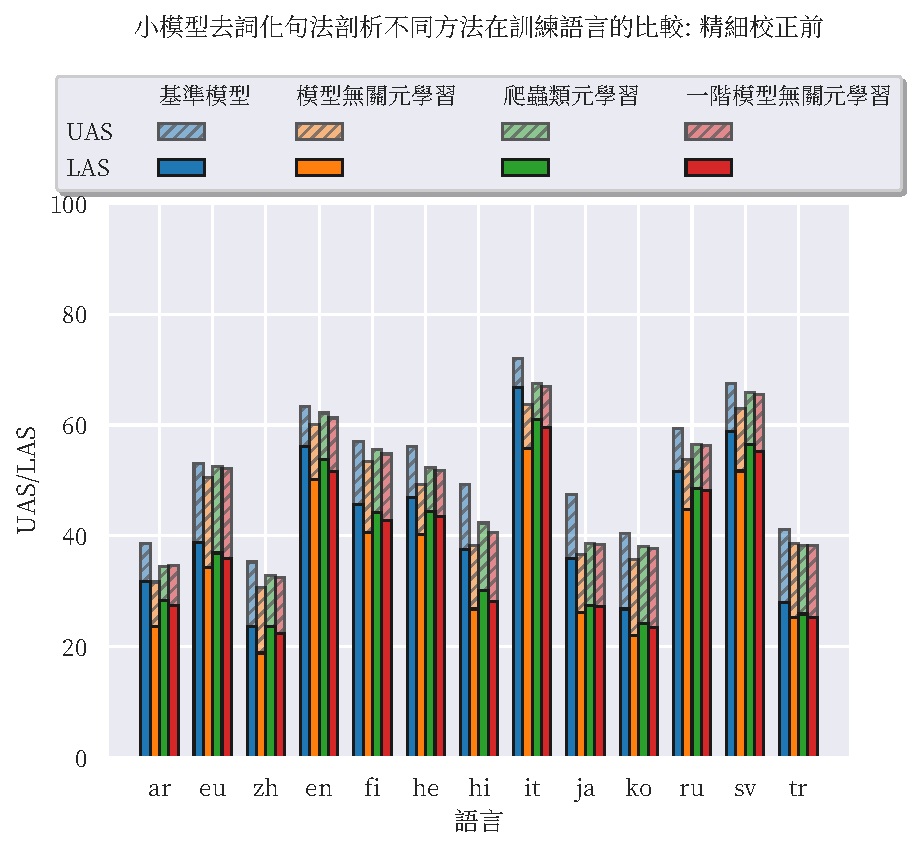
\includegraphics[width=\textwidth]{figs/delex_parsing/barplots/bar_small_zs_train_langs.pdf}
    \end{subfigure}
    \vspace{-12pt}
    \begin{subfigure}[t]{0.8\textwidth}
        \centering
        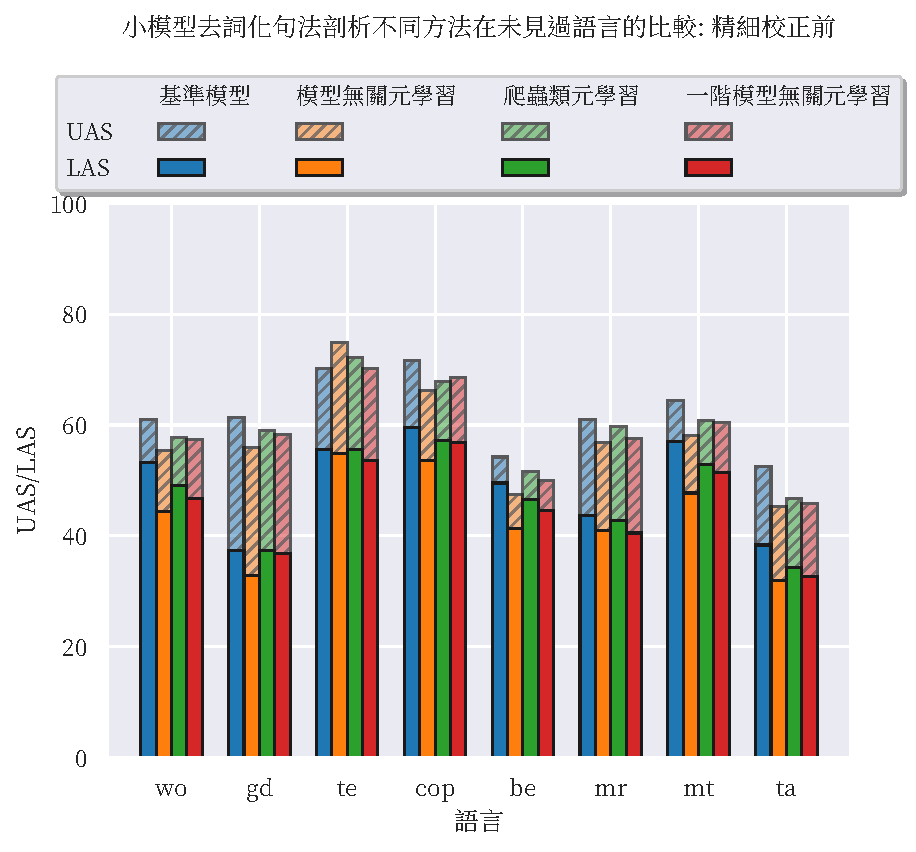
\includegraphics[width=\textwidth]{figs/delex_parsing/barplots/bar_small_zs_test_langs.pdf}
    \end{subfigure}
    \caption{小模型去詞化依存句法剖析不同方法在各語言精細校正前的UAS/LAS長條圖。}
    \label{fig:bar_small_zs}
\end{figure}
\begin{figure}[htbp]
    \centering
    \begin{subfigure}[t]{0.8\textwidth}
        \centering
        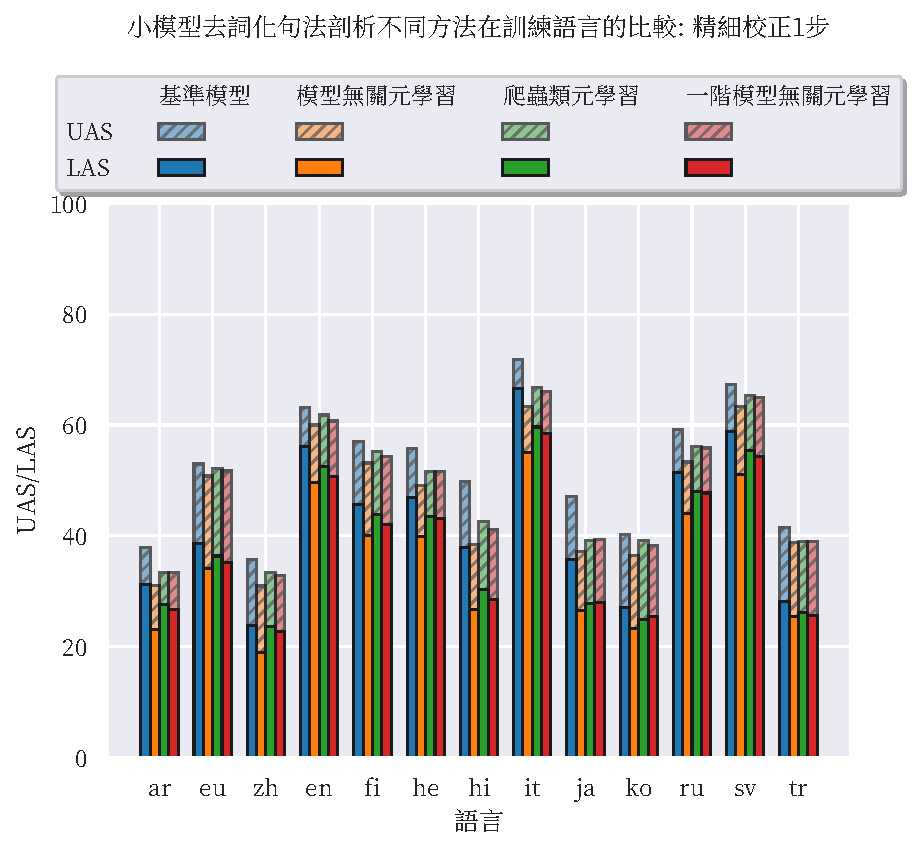
\includegraphics[width=\textwidth]{figs/delex_parsing/barplots/bar_small_one_step_train_langs.pdf}
    \end{subfigure}
    \vspace{-12pt}
    \begin{subfigure}[t]{0.8\textwidth}
        \centering
        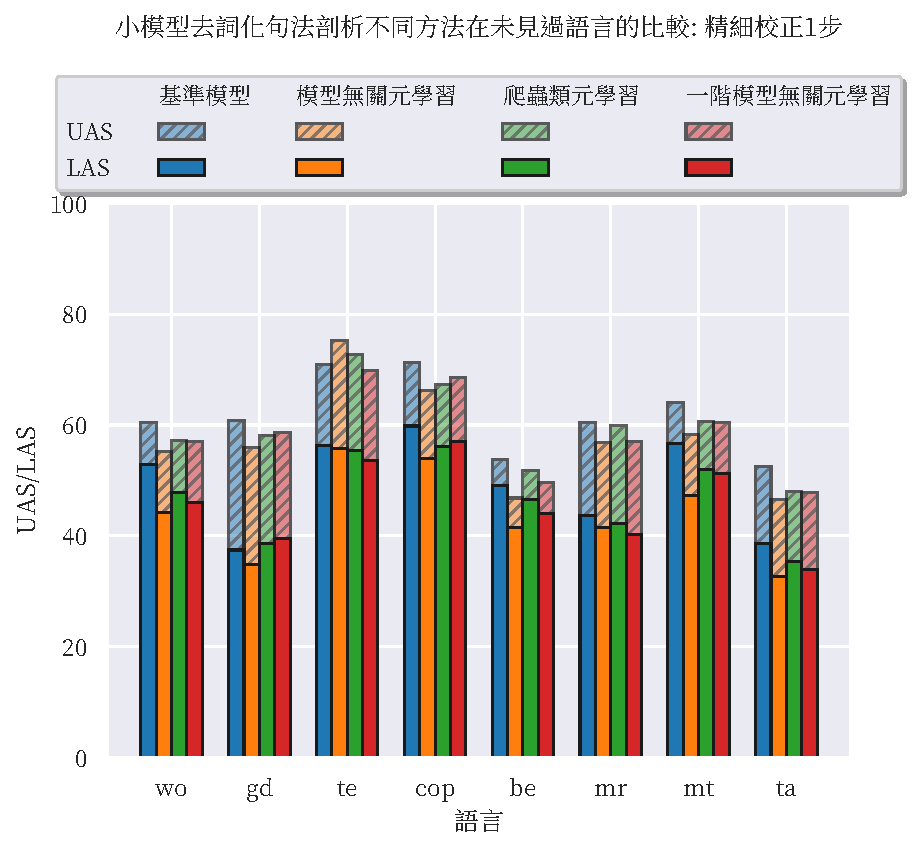
\includegraphics[width=\textwidth]{figs/delex_parsing/barplots/bar_small_one_step_test_langs.pdf}
    \end{subfigure}
    \caption{小模型去詞化依存句法剖析不同方法在各語言精細校正一步($\frac{1}{6}$回合)後的UAS/LAS長條圖。}
    \label{fig:bar_small_one_step}
\end{figure}
\begin{figure}[htbp]
    \centering
    \begin{subfigure}[t]{0.8\textwidth}
        \centering
        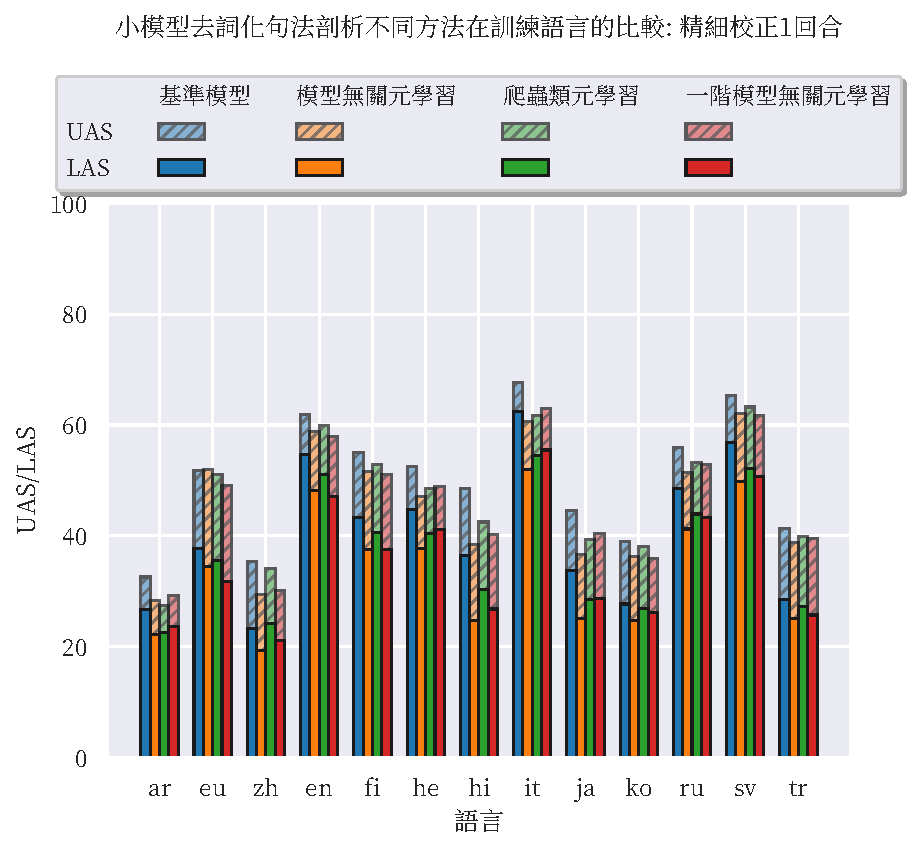
\includegraphics[width=\textwidth]{figs/delex_parsing/barplots/bar_small_full_epoch_1_train_langs.pdf}
    \end{subfigure}
    \vspace{-12pt}
    \begin{subfigure}[t]{0.8\textwidth}
        \centering
        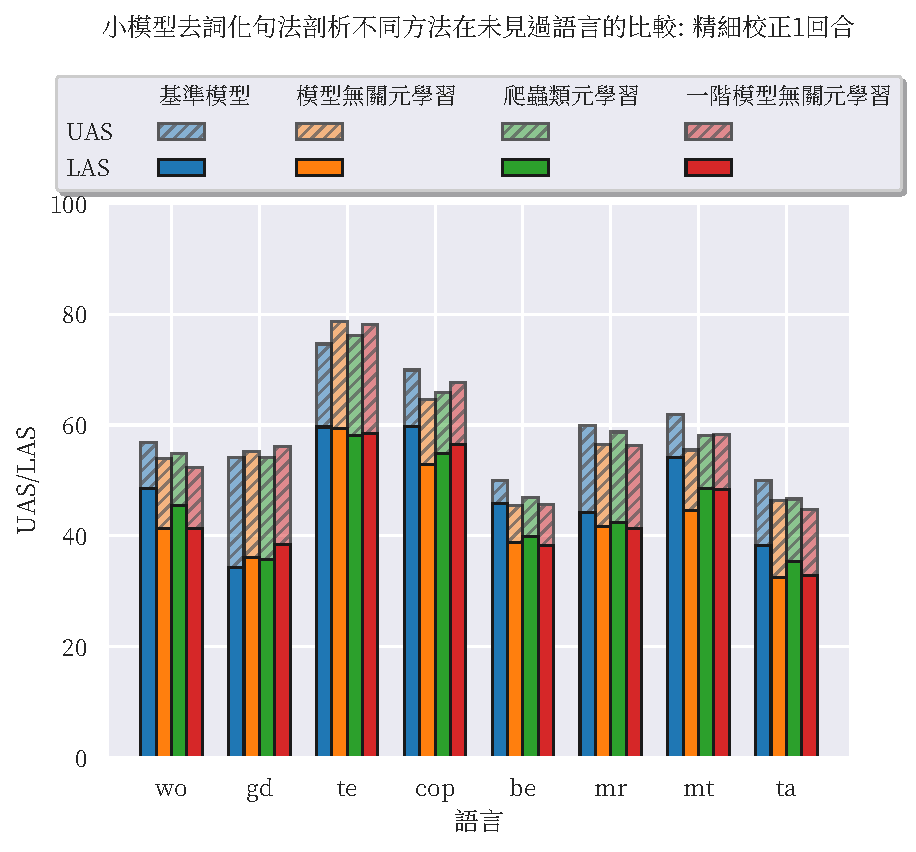
\includegraphics[width=\textwidth]{figs/delex_parsing/barplots/bar_small_full_epoch_1_test_langs.pdf}
    \end{subfigure}
    \caption{小模型去詞化依存句法剖析不同方法在各語言精細校正一回合後的UAS/LAS長條圖。}
    \label{fig:bar_small_full_epoch_1}
\end{figure}
\begin{figure}[htbp]
    \centering
    \begin{subfigure}[t]{0.8\textwidth}
        \centering
        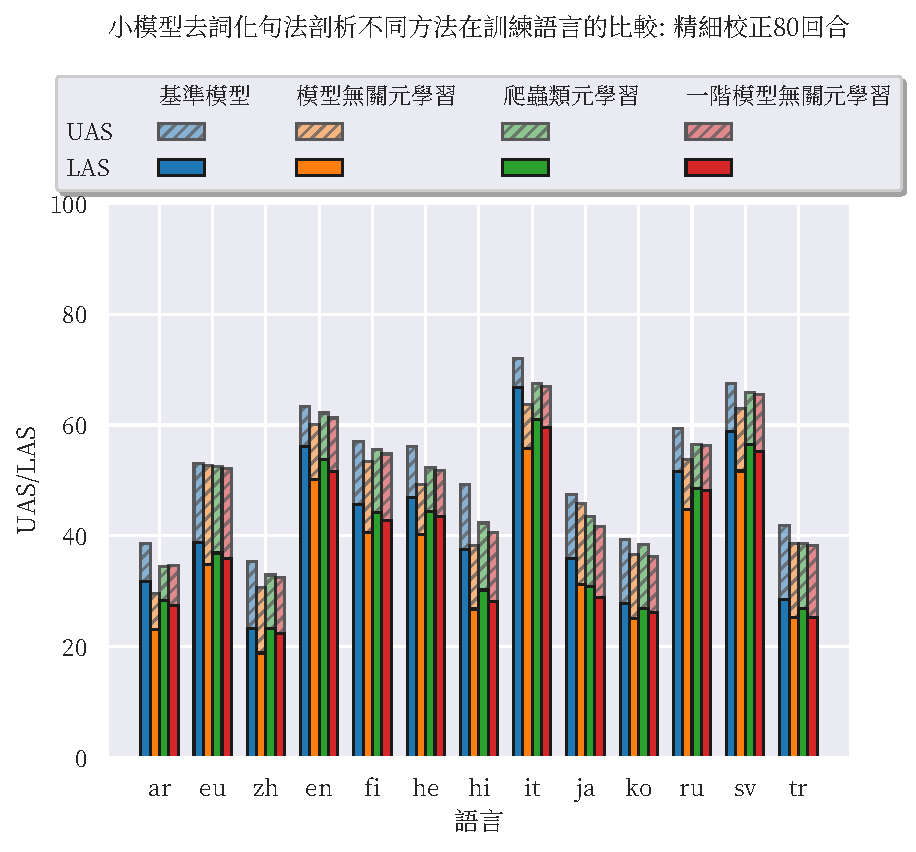
\includegraphics[width=\textwidth]{figs/delex_parsing/barplots/bar_small_full_epoch_80_train_langs.pdf}
    \end{subfigure}
    \vspace{-12pt}
    \begin{subfigure}[t]{0.8\textwidth}
        \centering
        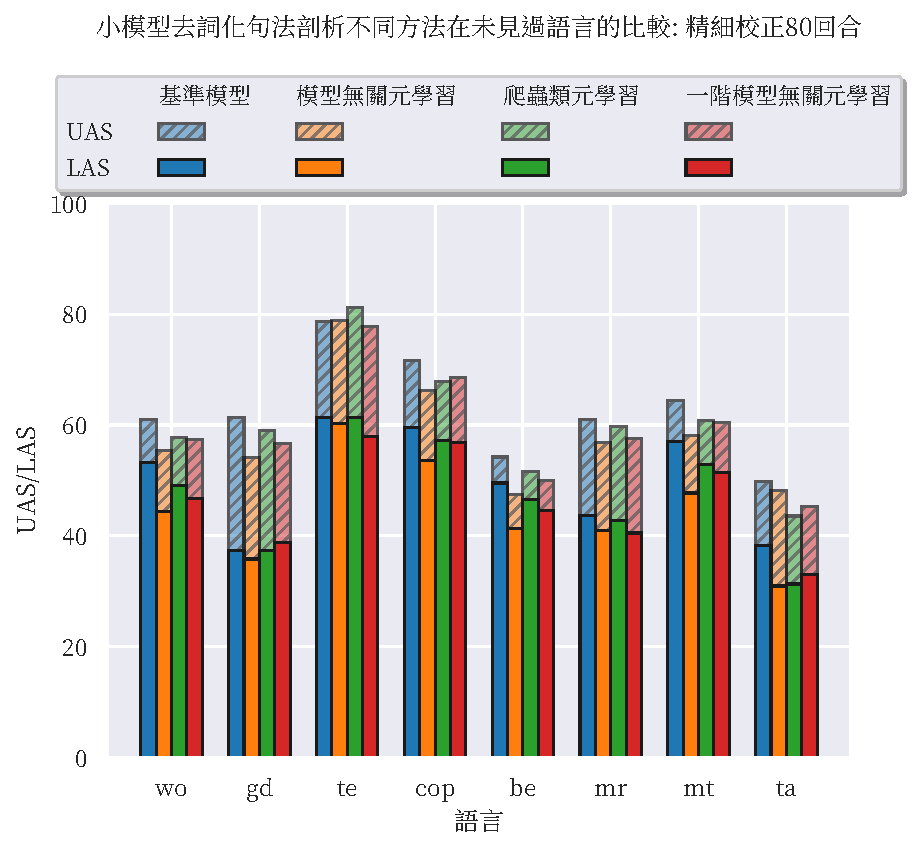
\includegraphics[width=\textwidth]{figs/delex_parsing/barplots/bar_small_full_epoch_80_test_langs.pdf}
    \end{subfigure}
    \caption{小模型去詞化依存句法剖析不同方法在各語言精細校正八十回合後的UAS/LAS長條圖。}
    \label{fig:bar_small_full_epoch_80}
\end{figure}

\begin{figure}[htbp]
    \centering
    \begin{subfigure}[t]{0.7\textwidth}
        \centering
        \includegraphics[width=\textwidth]{figs/delex_parsing/dir_scatterplots/small_zs_train_langs.pdf}
    \end{subfigure}
    \vspace{-12pt}
    \begin{subfigure}[t]{0.7\textwidth}
        \centering
        \includegraphics[width=\textwidth]{figs/delex_parsing/dir_scatterplots/small_zs_test_langs.pdf}
    \end{subfigure}
    \caption{小模型去詞化依存句法剖析不同方法在各語言精細校正前的方向性分佈。}
    \label{fig:small_dir_scatter_zs}
\end{figure}
\begin{figure}[htbp]
    \centering
    \begin{subfigure}[t]{0.7\textwidth}
        \centering
        \includegraphics[width=\textwidth]{figs/delex_parsing/dir_scatterplots/small_one_step_train_langs.pdf}
    \end{subfigure}
    \vspace{-12pt}
    \begin{subfigure}[t]{0.7\textwidth}
        \centering
        \includegraphics[width=\textwidth]{figs/delex_parsing/dir_scatterplots/small_one_step_test_langs.pdf}
    \end{subfigure}
    \caption{小模型去詞化依存句法剖析不同方法在各語言精細校正一步($\frac{1}{6}$回合)後的方向性分佈。}
    \label{fig:small_dir_scatter_one_step}
\end{figure}
\begin{figure}[htbp]
    \centering
    \begin{subfigure}[t]{0.7\textwidth}
        \centering
        \includegraphics[width=\textwidth]{figs/delex_parsing/dir_scatterplots/small_full_epoch_1_train_langs.pdf}
    \end{subfigure}
    \vspace{-12pt}
    \begin{subfigure}[t]{0.7\textwidth}
        \centering
        \includegraphics[width=\textwidth]{figs/delex_parsing/dir_scatterplots/small_full_epoch_1_test_langs.pdf}
    \end{subfigure}
    \caption{小模型去詞化依存句法剖析不同方法在各語言精細校正一回合後的方向性分佈。}
    \label{fig:small_dir_scatter_full_epoch_1}
\end{figure}
\begin{figure}[htbp]
    \centering
    \begin{subfigure}[t]{0.7\textwidth}
        \centering
        \includegraphics[width=\textwidth]{figs/delex_parsing/dir_scatterplots/small_full_epoch_80_train_langs.pdf}
    \end{subfigure}
    \vspace{-12pt}
    \begin{subfigure}[t]{0.7\textwidth}
        \centering
        \includegraphics[width=\textwidth]{figs/delex_parsing/dir_scatterplots/small_full_epoch_80_test_langs.pdf}
    \end{subfigure}
    \caption{小模型去詞化依存句法剖析不同方法在各語言精細校正八十回合後的方向性分佈。}
    \label{fig:small_dir_scatter_full_epoch_80}
\end{figure}

%\subsection{限制}
%去詞化依存句法剖析使用普適詞性標注在多語言句法剖析中,雖然排除了各個語言句法以外性質對句法剖析的影響


\iffalse
\begin{table}[htbp]
    \begin{subtable}[h]{0.8\textwidth}
        \centering
            \begin{tabular}[!ht]{c|llll}
                \hline
                語言 & 基準 & 模型無關元學習 & 爬蟲類元學習 & 一階模型無關元學習 \\
                \hline\hline
                wo & \textbf{62.83}** & 55.47 & \textbf{62.96}** & 45.69 \\
                gd & \textbf{44.47} & 37.42 & \textbf{44.14} & 34.97 \\
                te & 60.61 & 60.06 & \textbf{62.55} & 52.15 \\
                cop & \textbf{66.58} & 63.17 & \textbf{66.93} & 59.33 \\
                be & \textbf{71.87}** & 57.70 & 70.78 & 45.26 \\
                mr & \textbf{48.30}* & 42.48 & \textbf{47.33}* & 34.22 \\
                mt & \textbf{68.76}** & 61.77 & \textbf{68.42}** & 57.40 \\
                ta & 43.19 & 43.19 & \textbf{46.81}** & 32.73 \\
                \hline
                avg & 58.33 & 52.66 & \textbf{58.74} & 45.22 \\
                \hline
            \end{tabular}
            \caption{未精細校正(0回合)。}
    \end{subtable}
    \vfill
    \begin{subtable}[h]{0.8\textwidth}
        \centering
            \begin{tabular}[!ht]{c|llll}
                \hline
                語言 & 基準 & 模型無關元學習 & 爬蟲類元學習 & 一階模型無關元學習 \\
                \hline\hline
                wo & 63.64 & 63.91 & 63.39 & \textbf{64.22} \\
                gd & 46.49 & 45.87 & \textbf{47.96}* & 46.88 \\
                te & 64.36 & 65.05 & \textbf{65.60} & 62.55 \\
                cop & 67.03 & 66.99 & \textbf{67.44} & 66.93 \\
                be & \textbf{71.59}** & 69.13 & \textbf{71.11}** & 67.99 \\
                mr & 48.79 & \textbf{53.40}** & 47.57 & 48.54 \\
                mt & \textbf{68.84}* & 68.08 & \textbf{68.83}* & 68.04 \\
                ta & 45.35 & \textbf{50.48}** & 47.11 & 45.15 \\
                \hline
                avg & 59.51 & \textbf{60.36} & 59.88 & 58.79 \\
                \hline
            \end{tabular}
        \caption{精細校正1步($\frac{1}{6}$回合)。}
    \end{subtable}
    \vfill
    \begin{subtable}[h]{0.8\textwidth}
    \centering
        \begin{tabular}[!ht]{c|llll}
            \hline
            語言 & 基準 & 模型無關元學習 & 爬蟲類元學習 & 一階模型無關元學習 \\
            \hline\hline
            wo & 65.71 & 63.43 & \textbf{66.53}* & 61.40 \\
            gd & 53.79 & \textbf{57.30}** & \textbf{57.11}** & 55.74 \\
            te & 68.24 & 67.27 & \textbf{70.18} & 64.77 \\
            cop & 66.95 & 65.83 & \textbf{67.84}** & 64.86 \\
            be & \textbf{69.14}** & 65.57 & \textbf{69.51}** & 65.96 \\
            mr & 52.67 & \textbf{58.25} & 55.10 & 56.55 \\
            mt & \textbf{70.05}** & 67.33 & 69.20 & 66.83 \\
            ta & 51.58 & 53.75 & \textbf{54.35} & 53.49 \\
            \hline
            avg & 62.27 & 62.34 & \textbf{63.73} & 61.20 \\
            \hline
        \end{tabular}
        \caption{精細校正1回合。}
    \end{subtable}
    \vfill
    \begin{subtable}[h]{0.8\textwidth}
        \centering
            \begin{tabular}[!ht]{c|llll}
                \hline
                語言 & 基準 & 模型無關元學習 & 爬蟲類元學習 & 一階模型無關元學習 \\
                \hline\hline
                wo & \textbf{70.16}** & 67.08 & 68.80 & 67.12 \\
                gd & \textbf{65.33}** & 63.75 & \textbf{64.94}** & 63.19 \\
                te & 70.32 & \textbf{71.98} & 71.15 & 71.43 \\
                cop & \textbf{73.99}** & 72.37 & \textbf{74.05}** & 72.75 \\
                be & \textbf{71.87}** & 62.19 & 62.76 & 60.22 \\
                mr & 58.50 & \textbf{61.65} & 60.19 & 58.50 \\
                mt & \textbf{70.59}** & 67.86 & 69.49 & 67.43 \\
                ta & \textbf{61.64}** & 59.38 & 59.58 & 59.43 \\
                \hline
                avg & \textbf{67.80} & 65.78 & 66.37 & 65.01 \\
                \hline
            \end{tabular}
            \caption{精細校正80回合。}
        \end{subtable}
    \label{tab:delex_las_epoch_1}
    \caption{不同方法在未見過語言上精細校正不同回合後在測試集上的LAS之比較。\\
    ${ }^{**}$ $p < 0.001$ , ${ }^{*}$ $p < 0.01$。}
\end{table}
\begin{table}[htbp]
    \begin{subtable}[h]{0.8\textwidth}
        \centering
            \begin{tabular}[!ht]{c|llll}
                \hline
                語言 & 基準 & 模型無關元學習 & 模型無關元學習(4步) \\
                \hline\hline
                wo & \textbf{62.83}** & 55.47 & 44.66 \\
                gd & \textbf{44.47}** & 37.42 & 33.36 \\
                te & \textbf{60.61}* & \textbf{60.06}** & 56.03 \\
                cop & \textbf{66.58}** & 63.17 & 56.47 \\
                be & \textbf{71.87}** & 57.70 & 48.00 \\
                mr & \textbf{48.30}** & 42.48 & 39.56 \\
                mt & \textbf{68.76}** & 61.77 & 54.70 \\
                ta & \textbf{43.19}** & \textbf{43.19} & 35.95 \\
                \hline
                avg & \textbf{58.33} & 52.66 & 46.09 \\
                \hline
            \end{tabular}
            \caption{未精細校正(0回合)。}
    \end{subtable}
    \vfill
    \begin{subtable}[h]{0.8\textwidth}
        \centering
            \begin{tabular}[!ht]{c|lll}
                \hline
                語言 & 基準 & 模型無關元學習 & 模型無關元學習(4步) \\
                \hline\hline
                wo & 63.64 & \textbf{63.91} & 56.90 \\
                gd & \textbf{46.49} & 45.87 & 43.53 \\
                te & 64.36 & \textbf{65.05} & 60.33 \\
                cop & \textbf{67.03} & 66.99 & 64.78 \\
                be & \textbf{71.59} & 69.13 & 60.35 \\
                mr & 48.79 & \textbf{53.40} & 46.84 \\
                mt & \textbf{68.84} & 68.08 & 65.23 \\
                ta & 45.35 & \textbf{50.48} & 46.25 \\
                \hline
                avg & 59.51 & \textbf{60.36} & 55.53 \\
                \hline
            \end{tabular}
        \caption{精細校正1步($\frac{1}{6}$回合)。}
    \end{subtable}
    \vfill
    \begin{subtable}[h]{0.8\textwidth}
    \centering
        \begin{tabular}[!ht]{c|llll}
            \hline
            語言 & 基準 & 模型無關元學習 & 模型無關元學習(4步) \\
            \hline\hline
            wo & \textbf{65.71} & 63.43 & 63.77 \\
            gd & 53.79 & \textbf{57.30} & 56.34 \\
            te & 68.24 & 67.27 & \textbf{70.04} \\
            cop & \textbf{66.95} & 65.83 & 66.80 \\
            be & \textbf{69.14} & 65.57 & 64.47 \\
            mr & 52.67 & \textbf{58.25} & 57.52 \\
            mt & \textbf{70.05} & 67.33 & 68.35 \\
            ta & 51.58 & 53.75 & \textbf{55.05} \\
            \hline
            avg & 62.27 & 62.34 & \textbf{62.79} \\
            \hline
        \end{tabular}
        \caption{精細校正1回合。}
    \end{subtable}
    \vfill
    \begin{subtable}[h]{0.8\textwidth}
        \centering
            \begin{tabular}[!ht]{c|llll}
                \hline
                語言 & 基準 & 模型無關元學習 & 模型無關元學習(4步) \\
                \hline\hline
                wo & \textbf{70.16} & 67.08 & 66.45 \\
                gd & \textbf{65.33} & 63.75 & 63.73 \\
                te & 70.32 & \textbf{71.98} & 69.21 \\
                cop & \textbf{73.99} & 72.37 & 72.38 \\
                be & \textbf{71.87} & 62.19 & 66.64 \\
                mr & 58.50 & \textbf{61.65} & 61.41 \\
                mt & \textbf{70.59} & 67.86 & 68.18 \\
                ta & \textbf{61.64} & 59.38 & 59.38 \\
                \hline
                avg & \textbf{67.80} & 65.78 & 65.92 \\
                \hline
            \end{tabular}
            \caption{精細校正80回合。}
        \end{subtable}
    \label{tab:delex_las_epoch_1}
    \caption{不同步數的模型無關元學習在未見過語言上精細校正不同回合後在測試集上的LAS之比較。\\
    ${ }^{**}$ $p < 0.001$ , ${ }^{*}$ $p < 0.01$。}
\end{table}
\begin{table}[htbp]
    \begin{subtable}[h]{0.8\textwidth}
        \centering
            \begin{tabular}[!ht]{c|llll}
                \hline
                語言 & 基準 & 爬蟲類元學習 & 爬蟲類元學習(4步) \\
                \hline\hline
                wo & 62.83 & 62.96 & \textbf{63.98} \\
                gd & 44.47 & 44.14 & \textbf{44.48} \\
                te & 60.61 & \textbf{62.55} & 57.00 \\
                cop & 66.58 & \textbf{66.93} & 65.22 \\
                be & \textbf{71.87} & 70.78 & 70.49 \\
                mr & 48.30 & 47.33 & \textbf{49.27} \\
                mt & 68.76 & 68.42 & \textbf{69.24} \\
                ta & 43.19 & \textbf{46.81} & 44.39 \\
                \hline
                avg & 58.33 & \textbf{58.74} & 58.01 \\
                \hline
            \end{tabular}
            \caption{未精細校正(0回合)。}
    \end{subtable}
    \vfill
    \begin{subtable}[h]{0.8\textwidth}
        \centering
            \begin{tabular}[!ht]{c|lll}
                \hline
                語言 & 基準 & 爬蟲類元學習 & 爬蟲類元學習(4步) \\
                \hline\hline
                wo & 63.64 & 63.39 & \textbf{64.70} \\
                gd & 46.49 & \textbf{47.96} & 47.60 \\
                te & 64.36 & \textbf{65.60} & 62.14 \\
                cop & 67.03 & 67.44 & \textbf{67.83} \\
                be & \textbf{71.59} & 71.11 & 69.99 \\
                mr & 48.79 & 47.57 & \textbf{49.51} \\
                mt & 68.84 & 68.83 & \textbf{69.57} \\
                ta & 45.35 & 47.11 & \textbf{47.81} \\
                \hline
                avg & 59.51 & 59.88 & \textbf{59.89} \\
                \hline
            \end{tabular}
        \caption{精細校正1步($\frac{1}{6}$回合)。}
    \end{subtable}
    \vfill
    \begin{subtable}[h]{0.8\textwidth}
    \centering
        \begin{tabular}[!ht]{c|llll}
            \hline
            語言 & 基準 & 爬蟲類元學習 & 爬蟲類元學習(4步) \\
            \hline\hline
            wo & 65.71 & \textbf{66.53} & 66.08 \\
            gd & 53.79 & 57.11 & \textbf{57.66} \\
            te & 68.24 & \textbf{70.18} & 69.35 \\
            cop & 66.95 & 67.84 & \textbf{68.06} \\
            be & 69.14 & \textbf{69.51} & 67.10 \\
            mr & 52.67 & 55.10 & \textbf{55.83} \\
            mt & \textbf{70.05} & 69.20 & 69.79 \\
            ta & 51.58 & 54.35 & \textbf{56.31} \\
            \hline
            avg & 62.27 & 63.73 & \textbf{63.77} \\
            \hline
        \end{tabular}
        \caption{精細校正1回合。}
    \end{subtable}
    \vfill
    \begin{subtable}[h]{0.8\textwidth}
        \centering
            \begin{tabular}[!ht]{c|llll}
                \hline
                語言 & 基準 & 爬蟲類元學習 & 爬蟲類元學習(4步) \\
                \hline\hline
                wo & \textbf{70.16} & 68.80 & 68.98 \\
                gd & 65.33 & 64.94 & \textbf{65.37} \\
                te & 70.32 & 71.15 & \textbf{71.98} \\
                cop & 73.99 & 74.05 & \textbf{74.30} \\
                be & \textbf{71.87} & 62.76 & 68.04 \\
                mr & 58.50 & 60.19 & \textbf{61.65} \\
                mt & \textbf{70.59} & 69.49 & 69.24 \\
                ta & \textbf{61.64} & 59.58 & 60.73 \\
                \hline
                avg & \textbf{67.80} & 66.37 & 67.54 \\
                \hline
            \end{tabular}
            \caption{精細校正80回合。}
        \end{subtable}
    \label{tab:delex_las_epoch_1}
    \caption{不同步數的爬蟲類元學習在未見過語言上精細校正不同回合後在測試集上的LAS之比較。\\
    ${ }^{**}$ $p < 0.001$ , ${ }^{*}$ $p < 0.01$。}
\end{table}
\begin{table}[htbp]
    \begin{subtable}[h]{0.8\textwidth}
        \centering
            \begin{tabular}[!ht]{c|llll}
                \hline
                語言 & 基準 & 一階模型無關元學習 & 一階模型無關元學習(4步) \\
                \hline\hline
                wo & \textbf{62.83} & 45.69 & 4.24 \\
                gd & \textbf{44.47} & 34.97 & 5.48 \\
                te & \textbf{60.61} & 52.15 & 29.26 \\
                cop & \textbf{66.58} & 59.33 & 4.24 \\
                be & \textbf{71.87} & 45.26 & 3.72 \\
                mr & \textbf{48.30} & 34.22 & 17.72 \\
                mt & \textbf{68.76} & 57.40 & 5.88 \\
                ta & \textbf{43.19} & 32.73 & 7.19 \\
                \hline
                avg & \textbf{58.33} & 45.22 & 9.72 \\
                \hline
            \end{tabular}
            \caption{未精細校正(0回合)。}
    \end{subtable}
    \vfill
    \begin{subtable}[h]{0.8\textwidth}
        \centering
            \begin{tabular}[!ht]{c|lll}
                \hline
                語言 & 基準 & 一階模型無關元學習 & 一階模型無關元學習(4步) \\
                \hline\hline
                wo & 63.64 & \textbf{64.22} & 12.07 \\
                gd & 46.49 & \textbf{46.88} & 12.31 \\
                te & \textbf{64.36} & 62.55 & 50.07 \\
                cop & \textbf{67.03} & 66.93 & 23.00 \\
                be & \textbf{71.59} & 67.99 & 14.74 \\
                mr & \textbf{48.79} & 48.54 & 28.88 \\
                mt & \textbf{68.84} & 68.04 & 17.15 \\
                ta & \textbf{45.35} & 45.15 & 15.69 \\
                \hline
                avg & \textbf{59.51} & 58.79 & 21.74 \\
                \hline
            \end{tabular}
        \caption{精細校正1步($\frac{1}{6}$回合)。}
    \end{subtable}
    \vfill
    \begin{subtable}[h]{0.8\textwidth}
    \centering
        \begin{tabular}[!ht]{c|llll}
            \hline
            語言 & 基準 & 一階模型無關元學習 & 一階模型無關元學習(4步) \\
            \hline\hline
            wo & \textbf{65.71} & 61.40 & 60.92 \\
            gd & 53.79 & 55.74 & \textbf{56.18} \\
            te & \textbf{68.24} & 64.77 & 66.57 \\
            cop & 66.95 & 64.86 & \textbf{67.01} \\
            be & \textbf{69.14} & 65.96 & 61.62 \\
            mr & 52.67 & \textbf{56.55} & 56.55 \\
            mt & \textbf{70.05} & 66.83 & 65.94 \\
            ta & 51.58 & \textbf{53.49} & 50.28 \\
            \hline
            avg & \textbf{62.27} & 61.20 & 60.63 \\
            \hline
        \end{tabular}
        \caption{精細校正1回合。}
    \end{subtable}
    \vfill
    \begin{subtable}[h]{0.8\textwidth}
        \centering
            \begin{tabular}[!ht]{c|llll}
                \hline
                語言 & 基準 & 一階模型無關元學習 & 一階模型無關元學習(4步) \\
                \hline\hline
                wo & \textbf{70.16} & 67.12 & 65.39 \\
                gd & \textbf{65.33} & 63.19 & 62.81 \\
                te & 70.32 & \textbf{71.43} & 71.29 \\
                cop & \textbf{73.99} & 72.75 & 71.67 \\
                be & \textbf{71.87} & 60.22 & 59.43 \\
                mr & \textbf{58.50} & 58.50 & 57.28 \\
                mt & \textbf{70.59} & 67.43 & 66.80 \\
                ta & \textbf{61.64} & 59.43 & 58.87 \\
                \hline
                avg & \textbf{67.80} & 65.01 & 64.19 \\
                \hline
            \end{tabular}
            \caption{精細校正80回合。}
        \end{subtable}
    \label{tab:delex_las_epoch_1}
    \caption{不同步數的爬蟲類元學習在未見過語言上精細校正不同回合後在測試集上的LAS之比較。\\
    ${ }^{**}$ $p < 0.001$ , ${ }^{*}$ $p < 0.01$。}
\end{table}
\fi
